% THIS IS SIGPROC-SP.TEX - VERSION 3.1
% WORKS WITH V3.2SP OF ACM_PROC_ARTICLE-SP.CLS
% APRIL 2009
%
% It is an example file showing how to use the 'acm_proc_article-sp.cls' V3.2SP
% LaTeX2e document class file for Conference Proceedings submissions.
% ----------------------------------------------------------------------------------------------------------------
% This .tex file (and associated .cls V3.2SP) *DOES NOT* produce:
%       1) The Permission Statement
%       2) The Conference (location) Info information
%       3) The Copyright Line with ACM data
%       4) Page numbering
% ---------------------------------------------------------------------------------------------------------------
% It is an example which *does* use the .bib file (from which the .bbl file
% is produced).
% REMEMBER HOWEVER: After having produced the .bbl file,
% and prior to final submission,
% you need to 'insert'  your .bbl file into your source .tex file so as to provide
% ONE 'self-contained' source file.
%
% Questions regarding SIGS should be sent to
% Adrienne Griscti ---> griscti@acm.org
%
% Questions/suggestions regarding the guidelines, .tex and .cls files, etc. to
% Gerald Murray ---> murray@hq.acm.org
%
% For tracking purposes - this is V3.1SP - APRIL 2009

\documentclass{acm_proc_article-sp}
\usepackage{algorithm}
\usepackage{algpseudocode}
\usepackage{pifont}
\usepackage{url}
\begin{document}

\title{Parallelized Spectral Clustering on Apache Spark}

%
% You need the command \numberofauthors to handle the 'placement
% and alignment' of the authors beneath the title.
%
% For aesthetic reasons, we recommend 'three authors at a time'
% i.e. three 'name/affiliation blocks' be placed beneath the title.
%
% NOTE: You are NOT restricted in how many 'rows' of
% "name/affiliations" may appear. We just ask that you restrict
% the number of 'columns' to three.
%
% Because of the available 'opening page real-estate'
% we ask you to refrain from putting more than six authors
% (two rows with three columns) beneath the article title.
% More than six makes the first-page appear very cluttered indeed.
%
% Use the \alignauthor commands to handle the names
% and affiliations for an 'aesthetic maximum' of six authors.
% Add names, affiliations, addresses for
% the seventh etc. author(s) as the argument for the
% \additionalauthors command.
% These 'additional authors' will be output/set for you
% without further effort on your part as the last section in
% the body of your article BEFORE References or any Appendices.

\numberofauthors{3} %  in this sample file, there are a *total*
% of EIGHT authors. SIX appear on the 'first-page' (for formatting
% reasons) and the remaining two appear in the \additionalauthors section.
%
\author{
% You can go ahead and credit any number of authors here,
% e.g. one 'row of three' or two rows (consisting of one row of three
% and a second row of one, two or three).
%
% The command \alignauthor (no curly braces needed) should
% precede each author name, affiliation/snail-mail address and
% e-mail address. Additionally, tag each line of
% affiliation/address with \affaddr, and tag the
% e-mail address with \email.
%
% 1st. author
\alignauthor
Wenxuan Cai\\
       \affaddr{University of California}\\
       \affaddr{Berkeley, CA 94720}\\
       \email{wenxuancai@berkeley.edu}
% 2nd. author
\alignauthor
Yaohui Ye\\
       \affaddr{University of California}\\
       \affaddr{Berkeley, CA 94720}\\
       \email{yeyh@berkeley.edu}
       \alignauthor
Quan Peng\\
       \affaddr{University of California}\\
       \affaddr{Berkeley, CA 94720}\\
       \email{quan1992@berkeley.edu}
}
% There's nothing stopping you putting the seventh, eighth, etc.
% author on the opening page (as the 'third row') but we ask,
% for aesthetic reasons that you place these 'additional authors'
% in the \additional authors block, viz.

% Just remember to make sure that the TOTAL number of authors
% is the number that will appear on the first page PLUS the
% number that will appear in the \additionalauthors section.

\maketitle
\begin{abstract}
Clustering is one of the most popular techniques adopted in the industry and research area to detect group structure in the dataset. $k$-means and Spectral Clustering are two algorithms widely used for grouping similar subsets of data within a large dataset. $k$-means clustering is simple and fast, but depends heavily on the initialization and is likely to stuck on the local optimum. Spectral Clustering often outperforms $k$-means by using eigenvectors of the affinity matrix to project data into lower dimensions, and utilizes $k$-means clustering only on the last step of the algorithm. However, Spectral Clustering is computationally expensive and even the simple
 implementation has a serious memory bottleneck. Thus, in this project, we tried to run Spectral Clustering in parallel on Spark, with purpose 
to gain more insights into the performance of Spectral Clustering and study Spark, the most popular fast and general-purpose cluster computing system. In this project we experienced with Spectral Clustering on MNIST digit image dataset~\cite{Lichman:2013} and compared clustering speedup on different number of nodes. Specifically, we parallelzed different steps of Spectral Clustering and got a reasonably good speedup on 10,000 image dataset. Moreover, we tried different optimizations and measured how much they improved the clustering performance. For $k$-means, we tried smart initialization techniques such as KM-2~\cite{yan2009fast} and BF~\cite{bradley1998refining}. For Spectral Clustering, we applied subsampling at the beginning to group data points by a distortion minimizing transformation, and conducted Spectral Clustering on the preprocessed dataset~\cite{yan2009fast}. This optimization significantly reduced the time and memory needed by the algorithm while retaining comparable clustering accuracy. The combination of parallelism and algorithm optimizations provided us with a lot of speedup. From the project we got to learn how Spark works to achieven efficient parallelism, how to set up Spark cluster, and a nice way to parallelize Spectral Clustering on large dataset.
\end{abstract}

% A category with the (minimum) three required fields
\category{H.4}{Machine Learning}{Clustering}
%A category including the fourth, optional field follows...
\category{D.1.3}{Concurrent Programming}{Parallel programming}

\keywords{Machine Learning, $k$-means, Spectral Clustering, Spark} % NOT required for Proceedings

\section{Introduction}
Clustering is one of the most widely used techniques for exploratory data analysis,  with applications ranging from statistics, computer science, biology to social sciences and psychology~\cite{von2007tutorial}. Typical applications include graph partition, speech separation, and image segmentation. $k$-means is a  
clustering algorithm which is easy to implement. However, as we have worked with $k$-means over time, the simplest method doesn't always give the best clustering result. The performance of $k$-means can vary significantly depending on the initialization method. A lot of optimization techniques exist to solve this problem. For example, Hartigan proposed to run $k$-means for multiple time with random initializations and pick the best result~\cite{hartigan1979algorithm}. Sampling-based KM-2~\cite{yan2009fast} suggests to break the $k$-means into two steps. Before doing $k$-means on the entire data set, it would first run a quick $k$-means on a subset of data to pre-selected initialization centroids. 

While $k$-means provides reasonable clustering performance on most problems, 
Spectral Clustering, one of the most popular modern clustering algorithms, outperforms the traditional clustering algorithms such as $k$-means in finding group structure. The reason is that traditional $k$-means clustering only considers distances to cluster centroids, but Spectral Clustering utilizes the eigenvalues of the affinity matrix to perform dimensionality reduction and works with distance between all pairs of points. Spectral clustering has good performance on small data set but limited applicability to large-scale problems due to its computational complexity $O(n^3)$ in general, with $n$ data points. The reason is simple. Spectral Clustering requires to compute the similarity matrix of all data points, which is a $n$ by $n$ matrix. After that, doing the eigenvector decomposition is an operation of 
$O(n^3)$ complexity. This cubic runtime makes the algorithm prohibitively expensive on dataset of million level. In this project, we first implemented the basic Spectral Clustering algorithm. After that, we tried to run the algorithm in parallel on Spark to speedup runtime on large dataset. Morerover, we adopted the optimization technique from paper Fast Approximate Spectral Clustering \cite{yan2009fast} to speedup our Spectral Clustering. Given the complexity of the algorithm, it will be time-consuming to run on the large real world dataset. Taking usage of the parallelism and algorithmic optmization would allow us to train efficiently on more data and improve the result. Actually, we got comparable accuracy and faster runtime after applying all techniques. The remainder of the report is organized as follows. In Section 2, we will introduce the details of Speactral Clustering. In section 3, we decribe the ways that we parallelize different stages of Spark. In setion 4, we give an overview of Spark and our architecture. In section 6,  we evaluate our performances on testing set. We present the future work in section 7 and conclusion in Section 8.
%ACKNOWLEDGMENTS are optional

\section{Basic Clustering Algorithms}
\subsection{Spectral Clustering}
The goal of Spectral Clustering is to partition the data into k disjoint classes such that each point will be assigned to a single class. A good partition would break the data into several loosely connected components, while similarity within the component is high.

Basically, the Spectral Clustering is a flexible class of clustering procedures, which makes usage of the eigenvalue of the similarity matrix of the input data to perform dimensionality reduction before clustering in lower dimensions. Employing the eigenvector decomposition, Spectral Clustering is able to beat $k$-means when detecting group structures in data.

Before providing the algorithm in pseudocode, we would present the algorithm briefly and introduce our notations. Basically, Spectral Clustering can be divided into three steps, and each step possesses full potential for parallelization: Laplacian matrix construction, eigenvector decomposition, and clustering. Given $n$ data points $x_1, x_2, \cdots, x_n$ in $R^d$, the first step is to construct the affinity matrix $W$, where $W_{ij}$ is the distance between $x_i$ and $x_j$. In our case, we used the Euclidian distance directly. Thus $W_{ij} = \sqrt{\sum_{k=1}^d(x_{ik} - x_{jk})^2}$. As we computed the affinity matrix $W$, we then built the diagonal degree matrix $D$ where $D_{ii} = \sum_{k=1}^nW_{ik}$. With degree matrix, we computed the Laplacian Matrix $L = D - W$. After that, we took the first $k$ eigenvectors $u_1, u_2, \cdots, u_k$ of L, as matrix $U \in R^{n\times d}$. The last step was to use each row of $U$ as the a lower dimensional representation of $x_i$, and do a $k$-means clustering. 
Written in pseudocode, it is shown in Algorithm~\ref{algorithm_sc}.
\begin{algorithm}
\caption{Spectral Clustering}
\label{CHalgorithm}
\begin{algorithmic}[1]
\State Construct affinity matrix $W$ from data set $x_1, x_2, \cdots, x_n$
\State Construct degree matrix $D$ from $W$
\State $L \leftarrow D - W$
\State Build $U \in R^{n \times d}$ where the columns are the first $k$ eigenvectors of $L$ 
\State Use the $i^{th}$ row $U_i$ of $U$ to represent $x_i$, do $k$-means clusterings on $U_1, U_2, \cdots, U_n$
\end{algorithmic}
\label{algorithm_sc}
\end{algorithm}

\subsubsection{Bottleneck}
It can proved be proved that mathematically Spectral Clustering solves the Ncut problem. The algorithm is not hard to code, but there are two serious problems with the naive implementations.
\begin{enumerate}
\item{The memory overhead. Like PCA, spectral clustering takes usage of the spectrum of the affinity matrix to project data points into lower dimensions. Constructing affinity matrix on a single node requires $O(n^2)$ computation since it needs to process over all pairs of points. Consequently, we need to store the affinity matrix, which takes $O(n^2)$ space. Storing a dense matrix on a single machine RAM becomes impossible when $n$ goes to level of 100k. Using 32 bit integer, storing such an affinity matrix takes $(100,000^2) * 4 \textnormal{B} = 40 \textnormal{G}$ memory.
}
\item{The time complexity of Spectral Clustering is $O(n^3)$, which comes from the requirement to perform eigenvector decomposition on the $O(n^2)$ affinity matrix. To give the reader a quantified idea of this time lower bound, we ran the simple Spectral Clustering on the 10,000 images from MNIST digit dataset~\cite{Lichman:2013}. It took more than 30 minutes to do the eigenvector decomposition using the numpy library. Thus, Spectral Clustering is computationally expensive for large datasets, which limits its application to large-scale problems.}
\end{enumerate}

\subsubsection{Solution}
For the memory overhead, a lot of solutions exist to handle the memory bottleneck. Three typical ideas are
\begin{enumerate}
\item{Zero out $W_{ij}$ if it is smaller than a certain threshold $\epsilon$}
\item{For each point $x_i$, only store the k nearest neighbours in the affinity matrix}
\item{Use Nystrom approximation to store a dense submatrix~\cite{fowlkes2004spectral}}
\end{enumerate}
In our project, we chose the second solution. In theory, the smaller the $k$, the worse the result because we throw away more info. $k$ in $k$-nn is a tunable parameter, and we picked 500 which both fitted the memory of our machine and gave a good performance. 

In order to speedup the slow eigenvector decomposition, we adopted the idea from Michael Jordan's paper Fast Approximate Spectral Clustering ~\cite{yan2009fast} to do a downsampling at the beginning to significantly reduce the size of the affinity matrix. Basically, after choosing a sampling ratio $\alpha$, we first did a fast $k$-means on the data set to find $m = \alpha n$ centroids $y_1, y_2, \cdots, y_m$. Then, each $x_i$ will be represented by the centroid closest to it. Then we would perform the Spectral Clustering on $y_1, y_2, \cdots, y_m$, and recover the cluster membership for each $x_i$ by looking up the cluster membership of the corresponding $y$ centroid. This optimization turned out to work well, with a little drop in accuracy because we lost some information during the downsampling. Besides that, it significantly reduced the time and memory usage of the Spectral Clustering algorithm.

\subsection{$k$-means}
$k$-means is one of the most common clustering techniques. It aims at partitioning $n$ observations into $k$ clusters. The first step of this algorithm is to randomly choose $k$ points from the dataset as our initial cluster centroids. The second step is to take each point of the dataset and associate it to its nearest centroid. The third step is re-calculating the centroids for each cluster that we get from last step by taking the means of all points within that cluster. After calculating the $k$ new centroids, we calculate the new binding of each point and its nearest new centroid and start a new iteration from the second step. The algorithm stops when all centroids stop moving.

The accuracy of $k$-means is highly dependent on the initialization method, since if the initial centroids aren't well selected, the algorithm could be stuck on local optimum. Various approaches for selecting initial centroids have been proposed~\cite{kanungo2002efficient, arthur2007k, khan2004cluster}, and for our project, we used three different initialization methods, KM-1~\cite{hartigan1979algorithm}, KM-2~\cite{yan2009fast} and BF~\cite{bradley1998refining}, which will be described in following parts.

\subsubsection{Optimization - KM-1}
The first optimization is to simply run the algorithm for several times. For each time, we use randomly initialized centroids and calculate the accuracy after convergence. After repeating these runs, we choose the one with the highest accuracy as our final result.
\subsubsection{Optimization - KM-2}
KM-2 is the second optimization, which consists of two stages of $k$-means. During the first stage, we sample a fraction of the data uniformly at random and run $k$-means with $k$ clusters on the sampled data. The second stage uses the centroids obtained from the first stage as the initial centroids and run $k$-means. Basically, the idea is to obtain good initial centroids so that fewer iterations and restarts are needed for the second stage.
\subsubsection{Optimization - BF}
The Bradley and Fayyad algorithm (BF)~\cite{bradley1998refining} consists of three stages of $k$-means. At first, we run $k$-means on randomly selected subsets of the entire data set for several times. The output centroids of all individual runs form a new data set. In the second stage, we run $k$-means on the new data set and the obtained centroids are used as the initial cluster centers for the third stage of $k$-means.

\section{Parallel Spectral Clustering}
As we generalized Spectral Clustering into 3 steps: Laplacian Matrix Construction, Eigenvector Decomposition, $k$-means, we can use different method to parallelize each step.

\subsection{Parallel Laplacian Matrix Construction}
In order to speed up the similarity matrix construction, we adopted idea from Wen-Yen's paper~\cite{chen2011parallel} and used map and reduce operation on Spark to perform computation distributedly.

MapReduce is a parallel computing framework designed by Google~\cite{dean2008mapreduce}. Basically, it divides the computation jobs into two steps - the map phrase and reduce phrase. Programmer can pass in specific function to each phrase as long as it follows the general rule of MapReduce framework. In the map phrase, the function needs to map the input into key-value pairs, which would be shaffled afterwards and passed to the designated reducer. In the reduce phrase, key-value pairs which shared the same key are collected by a single reducer. The reduce funciton is responsible for processing these values and generate the final result. MapReduces offers an abstract programming model which is able to organize thousands of machiens to accomplish big parallel jobs. It also provides a fault tolerance mechinasm that starts redundent job on another node once it detects any job failure. In general, MapReduce is used in noniterative algorithms. In our case, computing Laplacian Matrix is an independent and noniterative job, which fits well into the spectiaty of MapReduce.

Spark provides an easy prgramming interface for launching MapReduce jobs. By passing a lambda expression, Spark is able to distribute RDD across partitions and collets result according to the user-specific reduce function. 

Because of the $O(n^2)$ memory overhead and the importance of using a sparse eigensolver, we chose to store only top 500 neighbours for each data point in the affinity matrix. In this case, with $p$ computing nodes, each node would store $n/p$ rows of affinity matrix. For the work, since for each data point we need to compute the distances to all other points, we partition the work as $n/p$ for each node. In the map phrase, based on the index $i$ of the mapper, it would scan through $in/p$ to $(i+1)n/p$ data points and emit the intermediate result with same key. Thus, each reducer can get a balanced amount of key/value paris and perform the distance computations. In the reduce phrase, each reducer would iterate through all its data points, and compute the distances to all other points. This requires some internodes communication and Spark handles that for us just like progmming distributed hashtable in UPC.

In order to take the top 500 neighbours for a data point, the simplest solution is to comptue all the n distances, sort them, and pick the top 500. This solves the problem but consumes lots of unnecessary memory to store all the $n$ distances, and this approach becomes expensive once $n$ gets large. Our solution here is to use a max heap, and keep the size to 500. In general, we keep $n/p$ max heaps. Whenever we read a remote points, we scan through the local points and put distances into corresponding max heap. This approach toook advantage of the locality and turned out to be much faster than fetching all remote points once for each local data point. Moreover, when computing distance $$||x_i - x_j|| = ||x_i||^2 + ||x_j||^2 - 2x_i^Tx_j$$
we cached the value of $|x_i||^2$ and $||x_j||^2$ and reuse them later. It gave us a much better $O(d)$ runtime. 

Since $k$ nearest neighobur is not a symmetric relationship, the affinity matrix we constructed is not going to be symmetric, which causes problem when passing to the sparse eigensolver later. We added a simple fix there that we copy each entry to its symmetric position in the matrix. After we computed the affinity matrix $W$, we constructed the diagnoal degree matrix $D$ and Laplacian matrix $L$ as 
$$ D_{ii} = \sum_{j=1}^nW_{ij}$$
$$ L = D - W$$

\subsection{Eigenvector Decomposition}
As we have the Laplacian matrix $L$, the next step is to find its eigenvetors to project data points into lower dimensions. A quick research through the existing sparase eigensolvers online pointed us to PARPACK~\cite{ding2011parallel}, a parallel ARPACK implementiation based on MPI.

MPI, known as message passing interface, is a cross platform message passing library for writing parallel programming. At the beginning, an MPI program will be loaded into the memory, and each processor / process will gain a unique ID. MPI provides a universal protocol for programs to exchagne messages and data. Different processes can communicate any synochornize with each other by calling MPI routines. Typical MPI functions are send, recv, broadcast, and reduce. PARPACK scales well on multiple nodes using MPI.

However, transforming PARPACK onto Spark would not be an easy thing to do, so we put our attentions to the existing MLlib (xxx) integrated with Spark, and we found the SVD implementation in Spark. SVD, short for Singular Value Decomposition, factorizes a matrix $X$ into the products of three matrices $$X = U\Sigma V^Y$$ where $U$ is the left singular matrix, $V$ is the right singular matrix, and $\Sigma$ is a diagnomal matrix of eigenvalues. The advantage of using Spark SVD is that we can specify the number of rank $k$ we want, so we don't have to compute all the eigenvectors and has a lower rank approximation to the original matrix. This can save storaage, reduce the communication cost, and reduce overfitting on aspect of machine learning. We used the SVD library call directly to compute the eigenvalue and eigenvectors of Laplacian matrix $L$. The current Spark SVD implementation in mllib is partially distributed. As we found from the source and document, the matrix-vector multipliation $X^TXv$ is computed in a distributed way, but the eigenvalues and eigenvectors are computed on the driver. Assume for a n by n matrix $X$, and we want the top $k$ eigenvectors, we need to fit a n by k matrix into driver's memory. Actually, behhind the screen, it calls the ARPACK to compute eigen-decomposition of $X^TX$ on the driver node. Although Spark SVD is not fully distributed at current version, we got enough memory on drive for our Amazon instance to finish the eigen-decomposition.


\subsection{Parallel $k$-means}
Once we get the first $k$ eigenvectors of the Laplacian matrix, we use $k$ means to process the matrix and each row of the matrix is regarded as one data point in the algorithm.

To parallelize $k$-means clustering, we first need to randomly select cluster centers from all points and then distribute all data points to different machines. At this point, each machine has a portion of the whole data set and a copy of cluster centroids. During each iteration, a node only needs to compute the new centroids information with local data thus parallelizing the algorithm. The model is very similar to MPI model as mentioned in \cite{chen2011parallel}, but the implementation of parallelization in Spark is making communication easier than MPI.


\section{Spark Overview}
Map/Reduce was first presented by Google in 2002~\cite{dean2008mapreduce} and has been widely used for processing large data sets in a distributed environment. However, when writing our own MR programs in Hadoop or R, we found it difficult both because of the complicated configuration of the system and the inflexibility for different problems. We always need to build specialized systems for different use cases, which limits its applications. Specialized systems, including Pregel~\cite{malewicz2010pregel} and  GraphLab~\cite{low2014graphlab}, were built to deal with some of the limitations of traditional Map/Reduce.

Hosted under Apache Open Source Licence, Spark is a fast and general-purpose clustering computer system which efficiently schedules parallelled jobs into distributed computation nodes and utilizes the in-memory cache to reduce IO communication overhead incurred in traditional Map/Reduce frameworks such as Hadoop~\cite{zaharia2010spark}. The goal of Spark is to generalize Map/Reduce to support new applications within the same engine. 

We chose Spark to be our parallelization tool for a couple of reasons. On the one hand, a lot of machine learning problems require iterative processing over training set to learn the best parameters, which typically applies the same function repeatedly. Traditional Map/Reduce framework saves the intermediate results onto disks and reads them back later if needed, which incurs unnecessary IO overhead. Spark, using fast in-memory cache for those intermediate values, avoids the performance penalty of data reload and speeds up the entire training process~\cite{zaharia2010spark}. On the other hand, we want to take the opportunity to experiment with this state-of-the-art technique and learn about how it works.

\begin{figure}[h]
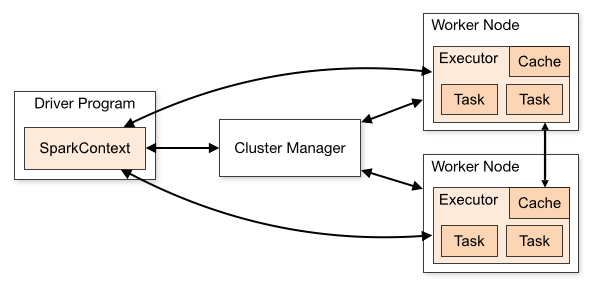
\includegraphics[height=4.1cm]{spark_architecture.png}
\caption{Spark Architecture~\cite{sparkoverview}}
\label{spark_arch}
\end{figure}

Figure~\ref{spark_arch} shows the architecture of a Spark system. Spark applications run as independent sets of processes on a cluster, coordinated by the SparkContext object in the main program~\cite{sparkoverview}. Spark uses a Master-Slave model, where the master node stores the SparkContext object and worker nodes (i.e., slave) are responsible for running computations and storing data for the application. When we want to run a Spark task, we can just submit it to the master node, and the SparkContext will send the tasks for the workers to run.

The most essential abstraction introduced by Spark is resilient distributed datasets (RDD), which is a collection of objects partitioned across different machines that enables Spark to perform efficient in-memory computation for iterative and interactive algorithms, which helped us a lot when running the experiments.

\section{Evaluation}
In this sector we present the dataset we tested on and the results from running different clustering algorithms with different numbers of computing nodes.

During evaluation, we used MNIST digit image dataset from \cite{mnistdigit}. In short, it consists of hand-written digit images in grey scale. Each image is 28 * 28, so we have 784 dimensions in total. Particularly, each dimension is a pixel of grey scale between 0 and 255. The 10,000 images we picked contains all digits from 0 to 9. Figure~\ref{visual_digits} gives the visualization of random images of different digits.

\begin{figure}[h]
\centering
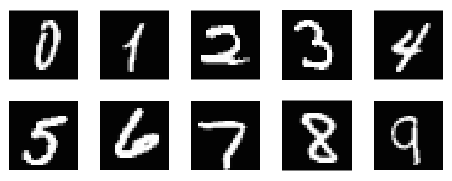
\includegraphics[height=3.2cm]{digits.png}
\caption{Visualization of digit images}
\label{visual_digits}
\end{figure}

\subsection{Environment}
We set up a Spark cluster of 8 nodes on Amazon Spot instances. One of these nodes is the Master node, which manages the tasks. The other 7 nodes are Workers, which are actually processes/processors that run computations and store data for the application. The spot instances we rent were R3.xlarge High Frequency Intel Xeon E5-2670 v2 (Ivy Bridge) Processors~\cite{spotinstance}, each of which has 4 VCPU and 27 GB of RAM. 

\subsection{Results}
We run our parallelized program with different number of workers, ranging from 1 to 7.

\subsubsection{Parallel Laplacian Matrix Construction}
In Table~\ref{table_lap}, we show the running time and speedup of the matrix construction with different node numbers on the MNIST digit dataset. In Figure~\ref{lm_time} we show the running time plot on different number of nodes and in Figure~\ref{lm_speedup} we show the speedup plot. We could observe that the matrix construction is expensive on a single node, and we gained around 5.3x speedup when processing on 7 nodes.

\begin{table}[h]
\centering
\begin{tabular}{|c|c|c|}
\hline
Nodes & Running time & Speedup \\
\hline
 1 & 1626.77s & - \\
 2 & 856.19s & 1.9\\
 3 & 580.99s & 2.8 \\
 4 & 464.79s & 3.5\\
 5 & 396.77s & 4.1\\
 6 & 346.12s & 4.7\\
 7 & 306.93s & 5.3\\
 \hline
\end{tabular}
\caption{Running time and Speedup of parallel Laplacian Matrix Construction on Spark}
\label{table_lap}
\end{table}

\begin{figure}[ht]
\centering
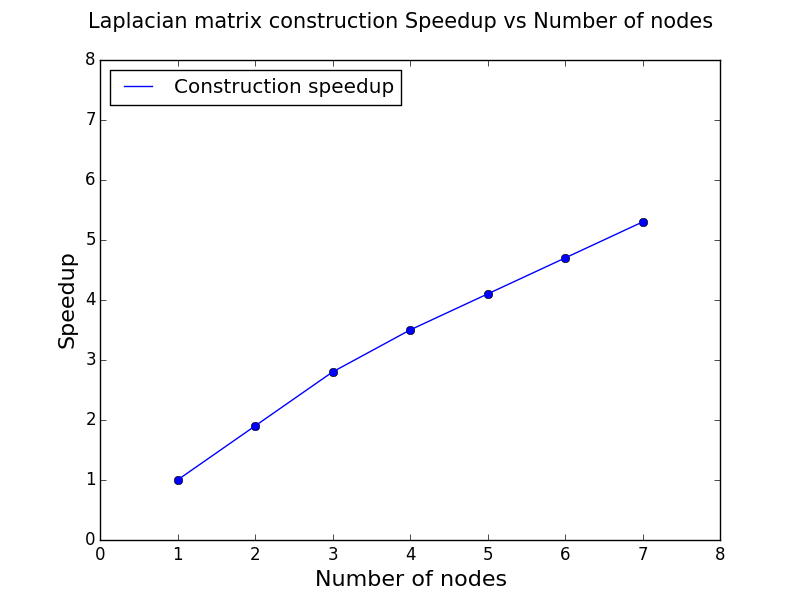
\includegraphics[height=6cm]{ms.png}
\caption{Laplacian matrix construction speedup vs number of nodes}
\label{lm_speedup}
\end{figure}

\begin{figure}[ht]
\centering
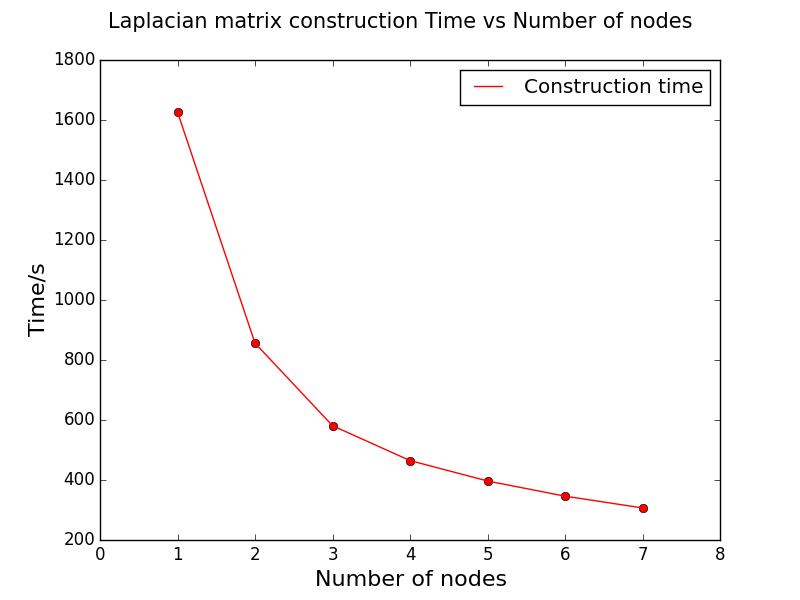
\includegraphics[height=6cm]{mt.png}
\caption{Laplacian matrix construction time vs number of nodes}
\label{lm_time}
\end{figure}

\subsubsection{Parallel $k$-means}
Table~\ref{table_kmeans} shows the running time and speedup of $k$-means clustering algorithm with different numbers of worker nodes. The speedup plot for the second part of the optimization, $k$-means clustering, is shown in Figure~\ref{km_speedup} and the corresponding time plot is shown in Figure~\ref{km_time}. We gained around 2.5x speedup of the algorithm with 7 nodes. Even though the speedup is still almost linear to the number of nodes, comparing with last experiment, it's actually further from the ideal speedup. We used our own $k$-means implementation, instead of using the MLlib one, thus it's possible that we failed to fully exploit the ability of Spark clusters.

\begin{table}[htb]
\centering
\begin{tabular}{|c|c|c|}
\hline
Nodes & Running time & Speedup \\
\hline
 1 & 27.35s & - \\
 2 & 21.20s & 1.3\\
 3 & 15.83s & 1.7 \\
 4 & 14.12s & 1.9\\
 5 & 13.52s & 2.0\\
 6 & 12.08s & 2.3\\
 7 & 11.00s & 2.5\\
 \hline
\end{tabular}
\caption{Running time and Speedup of parallel $k$-means on Spark}
\label{table_kmeans}
\end{table}

\begin{figure}[htb]
\centering
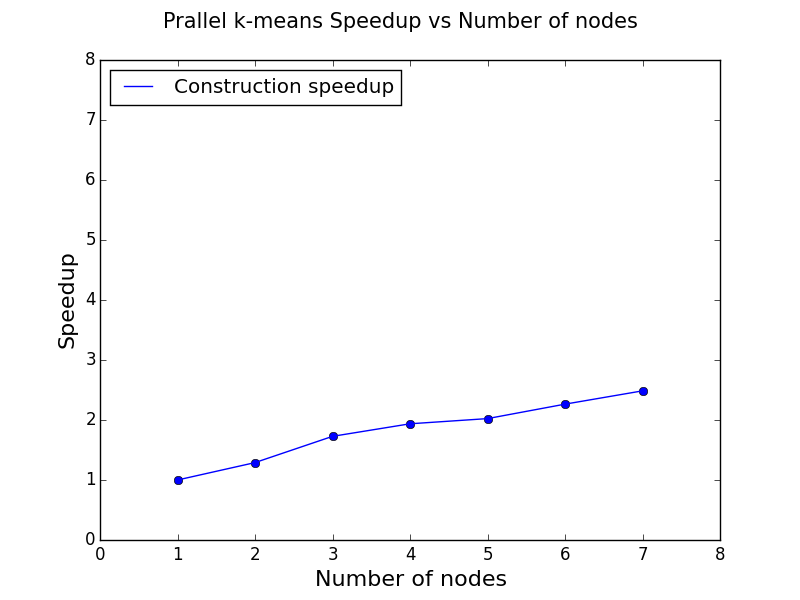
\includegraphics[height=6cm]{ks.png}
\caption{$k$-means convergence speedup vs number of nodes}
\label{km_speedup}
\end{figure}

\begin{figure}[htb]
\centering
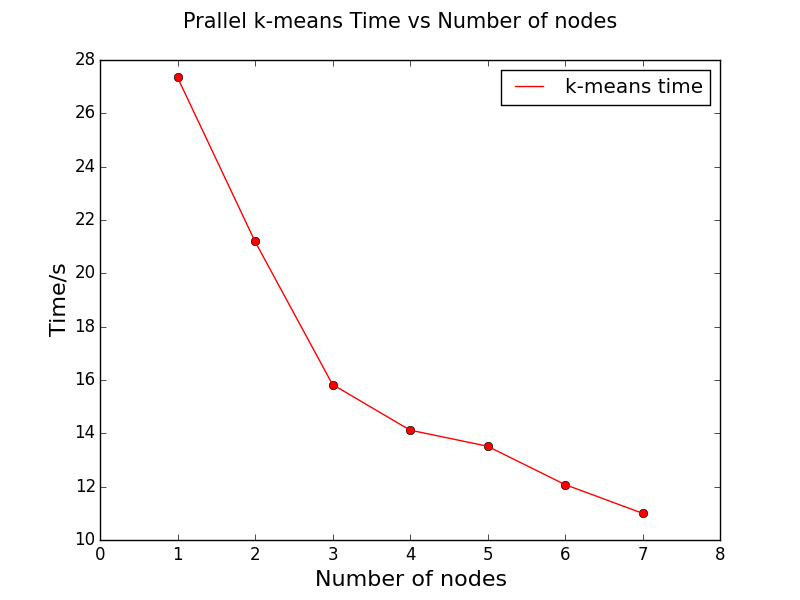
\includegraphics[height=6cm]{kt.png}
\caption{$k$-means convergence time vs number of nodes}
\label{km_time}
\end{figure}


\subsection{Centroids visualization}
Figure~\ref{visual_centroids} shows the visualization of the cluster centroids obtained from our Spectral Clustering algorithm, which successfully separated the boundry between different digit images.

\begin{figure}[ht]
\centering
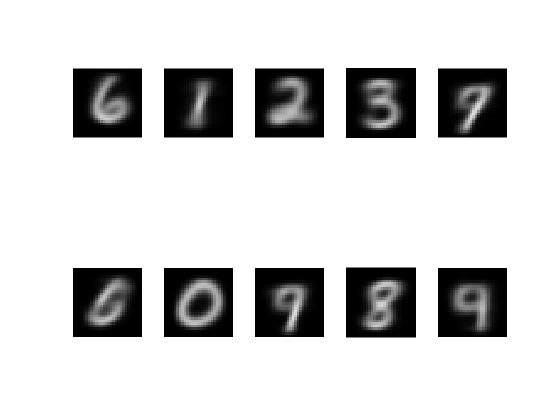
\includegraphics[height=3.2cm]{scdigits.png}
\caption{Visualization of cluster centroids}
\label{visual_centroids}
\end{figure}

\section{Future Work}
Currently we are using Eucledian distance in the affinity matrix. It provides a symmetric estimation of similarity, but is not the only choice for the distance metric. Other similarity metrics, such as Gaussian Kernel~\cite{keerthi2003asymptotic}, can be used to smooth the affinity estimation. Gaussian Kernel is defined as $$K(x, y) = \frac{|x - y|}{2\sigma^2}$$ $\sigma$ is a tunable parameters and it plays the role of smoothing the discision boundary. Adding the kernel could give us more complicated affinity metric and improve the performance.

For the eigenvector decomposition, we simply used the unnomarlized Laplacian Matrix $L = D - W$. Acturally, there exists other versions of the normalized Lapacian Matrix such as $L_{sym} = D^{-1/2}LD^{-1/2}$ and $L_{rw} = D^{-1}L$. As described by their names, $L_{sym}$ is a symmetric matrix, and $L_{rw}$ is closely related to random walk. The normalzied Laplacian matrix has some extra properties compared to unormalized one. Adding a distributed matrix multiplcation into our Spectral Clustering algorithm could help us explore these properties and see the influence on the final result.

Lastly, we could extend the project by applying parallel Spectral Clustering to other datasets such as bag-of-word~\cite{Lichman:2013} to cluster realted documents and compared results with other NLP models such as LDA~\cite{blei2003latent}.

\section{Conclusion}
In this project we experienced with Spectral Clustering algorithm. We started from the basic version of algorithm and parallelized the process on Spark. In short, compared to $k$-means which provides a fast clustering centroids searching technique, Spectral Clustering often gives much better results but has memory and runtime bottleneck for large dataset. The memory bottleneck happens when cosntructing the affinity matrix. We showed that use k nearest neighbour could effectively reduce the memory overhead, and other solutions exist such as threshold pruning or Nystrom approximation. We successfullly parallelized the Spectral Clustering to get speedup on multiple nodes on Spark. In this project, we parallelzed each stage of the algorithm. In short, we used MapReduce to build the affinity matrix in parallel; for the eigenvector decomposition, we took advantage of the existing Spark mllib library, which internally used ARPACK for fast computation; we distributed the computations of $k$-means on multiple nodes to get a faster converge. We also learned a lot of Spark during the project. It provided us with a friendly interface for running distributed jobs, and a good abstraction and scheduling of parallel workloads.

% The following two commands are all you need in the
% initial runs of your .tex file to
% produce the bibliography for the citations in your paper.
\bibliographystyle{abbrv}
\bibliography{citations}  % sigproc.bib is the name of the Bibliography in this case
% You must have a proper ".bib" file
%  and remember to run:
% latex bibtex latex latex
% to resolve all references
%
% ACM needs 'a single self-contained file'!
%
%APPENDICES are optional
%\balancecolumns

\balancecolumns
% That's all folks!
\end{document}


